\section{Survey of approximate matching techniques}
As far as we can see, approximate matching is in general more complicated than exact matching. We can consider exact matching problems as a subset of approximate matching problems with an error of 0. The time complexity of many effcient exact matching algorithms that work as simulating a DFA, such as Knuth–Morris–Pratt, will become exponential as the number of errors grows if we just convert the NFA of the pattern into a DFA to be adapted in these algorithms. 

\begin{comment}

\subsection{Dynamic programming}

One of the classical solutions to approximate matching problem is to use dynamic programming. This method is simple and easy to be implemented by programming. 

% TODO: some examples maybe


\subsection{Autamata simulation}
Another classical one is automata simulation. The algortihm BNDM  (we will explain later) over which NR-grep is built is basically a simulation of an NFA. 

\end{comment}


\subsection{NR-grep}
From the experiment results shown in the previous section, we can say in general NR-grep has the best performance in average in our various test cases. This is not surprising because NR-grep implemented different efficient algorithms for various pattern matching problems as well as a good software design. From this tool's perspective, the patterns are classified into three levels: simple patterns, extended patterns and regular experssions. Different algorithms are applied to different levels of patterns to make sure that the problem can be solved in the most efficient way. 

We now show the idea of how NR-grep solves the approximate matching in an efficient way. The name of this tool comes from "nondeterministic reverse $grep$", which indicates this tool can simulate NFAs instead of converting them to DFAs. The algorithm of  simulating NFAs used in NR-grep is called $Shift-Or$. This algorithm is based on an approach called $bit-parallelism$, which takes advantage of the parallelism of the bit operations inside a computer word. A variant of Shift-Or that is easier to explain is $Shift-And$ algorithm, which also based on $bit-parallelism$. We first show how this algorithm works. 

Given a pattern $pat$ of length $m$,  and a text $txt$ of length $n$ and the alphabet set is $\Sigma$ with a size $|\Sigma|$. First we build a table $B$ in which for each character in $\Sigma$ stores a bit mask $b_m...b_1$. Each bit mask in the table has a length of $m$. For a character $char$ in $pat$ with an index $i$ (1-indexed), set the $m-i-1$ bit of the mask in B[$char$]. The following example shows a bit mask table for the pattern "abc" assuming $\Sigma$ = {a,b,c,d}.


\begin{example}\emph{The bit mask table for pattern "abc".}

\begin{table}[H]
	\centering
	\begin{tabular}{|c|c|c|c|}
		\hline
		index      & 1                        & 2                        & 3                        \\ \hline
		\textbf{a} & 0                        & 0                        & {\color[HTML]{3531FF} 1} \\ \hline
		\textbf{b} & 0                        & {\color[HTML]{3531FF} 1} & 0                        \\ \hline
		\textbf{c} & {\color[HTML]{3531FF} 1} & 0                        & 0                        \\ \hline
		\textbf{d} & 0                        & 0                        & 0                        \\ \hline
	\end{tabular}
	\label{table-bitmask}
\end{table}
\end{example}

An NFA that can be used to search for this pattern in a text is as follows.

\begin{figure}[H]
\centering
	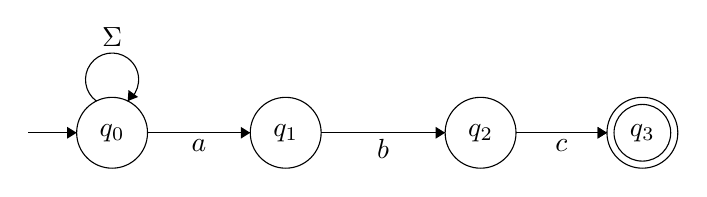
\begin{tikzpicture}[scale=0.15]
	\tikzstyle{every node}+=[inner sep=0pt]
	\draw [black] (18.3,-25.8) circle (3);
	\draw (18.3,-25.8) node {$q_0$};
	\draw [black] (49.5,-25.8) circle (3);
	\draw (49.5,-25.8) node {$q_2$};
	\draw [black] (33,-25.8) circle (3);
	\draw (33,-25.8) node {$q_1$};
	\draw [black] (63.2,-25.8) circle (3);
	\draw (63.2,-25.8) node {$q_3$};
	\draw [black] (63.2,-25.8) circle (2.4);
	\draw [black] (11.2,-25.8) -- (15.3,-25.8);
	\fill [black] (15.3,-25.8) -- (14.5,-25.3) -- (14.5,-26.3);
	\draw [black] (21.3,-25.8) -- (30,-25.8);
	\fill [black] (30,-25.8) -- (29.2,-25.3) -- (29.2,-26.3);
	\draw (25.65,-26.3) node [below] {$a$};
	\draw [black] (36,-25.8) -- (46.5,-25.8);
	\fill [black] (46.5,-25.8) -- (45.7,-25.3) -- (45.7,-26.3);
	\draw (41.25,-26.3) node [below] {$b$};
	\draw [black] (16.977,-23.12) arc (234:-54:2.25);
	\draw (18.3,-18.55) node [above] {$\Sigma$};
	\fill [black] (19.62,-23.12) -- (20.5,-22.77) -- (19.69,-22.18);
	\draw [black] (52.5,-25.8) -- (60.2,-25.8);
	\fill [black] (60.2,-25.8) -- (59.4,-25.3) -- (59.4,-26.3);
	\draw [black] (52.5,-25.8) -- (60.2,-25.8);
	\fill [black] (60.2,-25.8) -- (59.4,-25.3) -- (59.4,-26.3);
	\draw (56.35,-26.3) node [below] {$c$};
	\end{tikzpicture}
\caption{A NFA to search for the pattern "abc".}
\end{figure}

We use a computer word $D = d_m...d_1$ to store the current active state in this NFA with an initial value of all bits 0. During the simulation, $D$ is updated with the following formula: 
$$D \leftarrow ((D << 1) \ | \ 0^{m-1}1) \ \& \ B[t_j]$$
where $t_j$ is the next text character.  When the $d_m$ bit in $D$ is set, we report the match. 

One of the advantages of the $Shift-Or$ algorithm is that it is easy to be extended to handle classes of characters, which is helpful for approximate matching. 

For example, we can now search the pattern "ab\{c|d\}" with almost the same time complexity as search "abc". The new bit mask table as Example \ref{table-bitmask2} shows just needs to set the first bit of the character $b$. 

\begin{example}\emph{The bit mask table for pattern "ab\{c|d\}"}.
	\begin{table}[H]
		\centering
		\begin{tabular}{|c|c|c|c|}
			\hline
			index      & 1                        & 2                        & 3                        \\ \hline
			\textbf{a} & 0                        & 0                        & {\color[HTML]{3531FF} 1} \\ \hline
			\textbf{b} &  {\color{red} 1}                    & {\color[HTML]{3531FF} 1} & 0                        \\ \hline
			\textbf{c} & {\color[HTML]{3531FF} 1} & 0                        & 0                        \\ \hline
			\textbf{d} & 0                        & 0                        & 0                        \\ \hline
		\end{tabular}
		\label{table-bitmask2}
	\end{table}
\end{example}
 


\begin{center}
	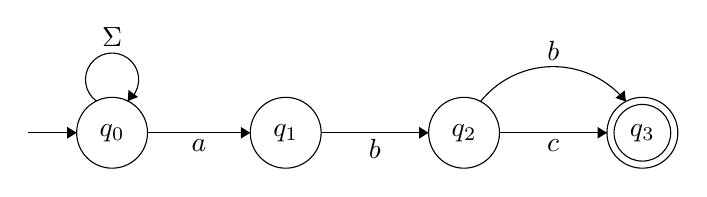
\begin{tikzpicture}[scale=0.15]
	\tikzstyle{every node}+=[inner sep=0pt]
	\draw [black] (18.3,-25.8) circle (3);
	\draw (18.3,-25.8) node {$q_0$};
	\draw [black] (33,-25.8) circle (3);
	\draw (33,-25.8) node {$q_1$};
	\draw [black] (63.2,-25.8) circle (3);
	\draw (63.2,-25.8) node {$q_3$};
	\draw [black] (63.2,-25.8) circle (2.4);
	\draw [black] (48.1,-25.8) circle (3);
	\draw (48.1,-25.8) node {$q_2$};
	\draw [black] (11.2,-25.8) -- (15.3,-25.8);
	\fill [black] (15.3,-25.8) -- (14.5,-25.3) -- (14.5,-26.3);
	\draw [black] (21.3,-25.8) -- (30,-25.8);
	\fill [black] (30,-25.8) -- (29.2,-25.3) -- (29.2,-26.3);
	\draw (25.65,-26.3) node [below] {$a$};
	\draw [black] (16.977,-23.12) arc (234:-54:2.25);
	\draw (18.3,-18.55) node [above] {$\Sigma$};
	\fill [black] (19.62,-23.12) -- (20.5,-22.77) -- (19.69,-22.18);
	\draw [black] (36,-25.8) -- (45.1,-25.8);
	\fill [black] (45.1,-25.8) -- (44.3,-25.3) -- (44.3,-26.3);
	\draw (40.55,-26.3) node [below] {$b$};
	\draw [black] (49.489,-23.161) arc (141.34482:38.65518:7.889);
	\fill [black] (61.81,-23.16) -- (61.7,-22.22) -- (60.92,-22.85);
	\draw (55.65,-19.7) node [above] {$b$};
	\draw [black] (51.1,-25.8) -- (60.2,-25.8);
	\fill [black] (60.2,-25.8) -- (59.4,-25.3) -- (59.4,-26.3);
	\draw (55.65,-26.3) node [below] {$c$};
	\end{tikzpicture}
\end{center}


\subsection{Python (\texttt{regex})}

\subsection{Scan For Matches}


\subsection{Approximate Kleenex}